\subsection*{Problema 05}

\textbf{Enunciado:} \\
Calcular la siguiente integral indefinida:
\begin{align*}
\int \dfrac{2x - 3}{x^2 + 6x + 15} \, dx
\end{align*}

\textbf{Solución:} \\
Para resolver esta integral, buscamos en el numerador la derivada del denominador. 
El denominador es $u = x^2 + 6x + 15$, cuya derivada es $u' = 2x + 6$.

Manipulamos algebraicamente el numerador para que aparezca dicha derivada:
\begin{align*}
2x - 3 &= (2x + 6) - 6 - 3 \\
&= (2x + 6) - 9
\end{align*}

Sustituimos esto en la integral original y separamos en dos integrales:
\begin{align*}
&\int \dfrac{2x - 3}{x^2 + 6x + 15} \, dx = \\
&\int \dfrac{2x + 6}{x^2 + 6x + 15} \, dx - 9 \int \dfrac{1}{x^2 + 6x + 15} \, dx
\end{align*}

Resolvemos la primera integral usando sustitución $u = x^2 + 6x + 15$, $du = (2x + 6) \, dx$:
\begin{align*}
\int \dfrac{2x + 6}{x^2 + 6x + 15} \, dx &= \ln|x^2 + 6x + 15|
\end{align*}

Para la segunda integral, completamos el trinomio cuadrado perfecto en el denominador:
\begin{align*}
x^2 + 6x + 15 &= (x^2 + 6x + 9) + 6 \\
&= (x + 3)^2 + (\sqrt{6})^2
\end{align*}

Aplicamos la fórmula de integración para la arcotangente:
\begin{align*}
&\int \dfrac{1}{(x + 3)^2 + (\sqrt{6})^2} \, dx \\
&= \dfrac{1}{\sqrt{6}} \arctan\left(\dfrac{x + 3}{\sqrt{6}}\right)
\end{align*}

Combinando ambos resultados y añadiendo la constante de integración $C$, obtenemos la solución final:
\begin{align*}
\int &\dfrac{2x - 3}{x^2 + 6x + 15} \, dx = \\
&\ln|x^2 + 6x + 15| \\
&- \dfrac{9}{\sqrt{6}} \arctan\left(\dfrac{x + 3}{\sqrt{6}}\right) + C
\end{align*}

\begin{figure}[H]
	\centering
	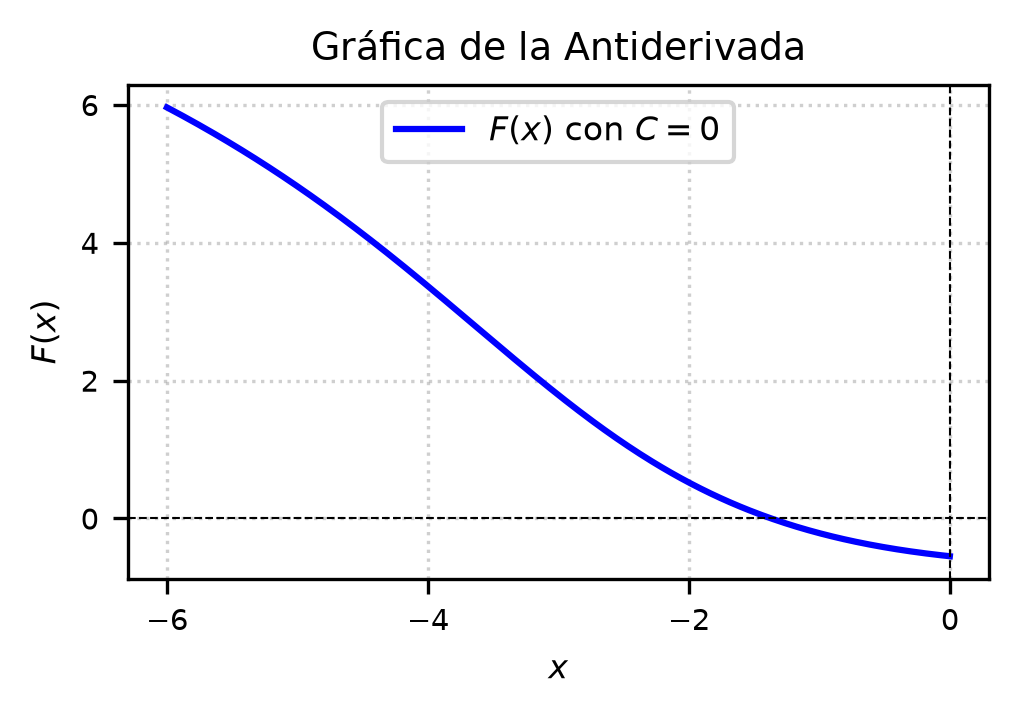
\includegraphics[width=\columnwidth]{semana_03/graficas/SEM03_P05_grafica.png}
	\caption{Representación gráfica de $f(x)$ y su antiderivada $F(x)$ evaluada para la constante de integración $C = 0$ (Problema 05).}
	\label{fig:problema05}
\end{figure}
